\documentclass[12pt,a4paper]{article}

% --- Packages ---
\usepackage[utf8]{inputenc}
\usepackage[T5]{fontenc}
\usepackage[vietnamese]{babel}
\usepackage{amsmath,amsfonts,amssymb}
\usepackage{graphicx}
\usepackage{hyperref}
\usepackage{geometry}
\usepackage{booktabs}
\usepackage{float}
\usepackage{array}
\usepackage{longtable}
\usepackage{fancyhdr}
\usepackage{titlesec}
\usepackage{subcaption}

% --- Cấu hình Trang giấy ---
\geometry{
    left=3cm,
    right=2cm,
    top=2.5cm,
    bottom=2.5cm,
}

% --- Cấu hình Header và Footer ---
\pagestyle{fancy}
\fancyhf{}
\fancyhead[L]{\small Báo cáo Đồ án Cuối kỳ - Thực hành NLP}
\fancyhead[R]{\small Sinh viên: Nguyễn Phúc Bách - 23280039}
\fancyfoot[C]{\thepage}
\renewcommand{\headrulewidth}{0.4pt}
\renewcommand{\footrulewidth}{0pt}

% --- Cấu hình định dạng Tiêu đề ---
\titleformat{\section}{\normalfont\Large\bfseries}{\thesection.}{1em}{}
\titleformat{\subsection}{\normalfont\large\bfseries}{\thesubsection.}{1em}{}
\titleformat{\subsubsection}{\normalfont\normalsize\bfseries}{\thesubsubsection.}{1em}{}

% --- Cấu hình Hyperref ---
\hypersetup{
    colorlinks=true,
    linkcolor=blue,
    filecolor=magenta,      
    urlcolor=cyan,
    pdftitle={Báo cáo Đồ án Cuối kỳ - Phân tích cảm xúc Shopee},
    pdfauthor={Nguyễn Phúc Bách - 23280039},
}

\begin{document}

% ==========================================
% TRANG BÌA CHUYÊN NGHIỆP
% ==========================================
\begin{titlepage}
    \centering
    \vspace*{1cm}
    
    {\large \textbf{ĐẠI HỌC QUỐC GIA THÀNH PHỐ HỒ CHÍ MINH}}\\[0.2cm]
    {\large \textbf{TRƯỜNG ĐẠI HỌC KHOA HỌC TỰ NHIÊN}}\\[0.2cm]
    {\large \textbf{KHOA CÔNG NGHỆ THÔNG TIN}}\\[1.5cm]
    
    \begin{figure}[H]
        \centering
        \vspace{1cm}
    \end{figure}
    
    {\Large \textbf{BÁO CÁO ĐỒ ÁN CUỐI KỲ}}\\[0.4cm]
    {\LARGE \textbf{MÔN HỌC: THỰC HÀNH XỬ LÝ NGÔN NGỮ TỰ NHIÊN}}\\[1.5cm]
    
    \rule{\textwidth}{1.5pt}\\[0.5cm]
    {\Large \bfseries ĐỀ TÀI: NGHIÊN CỨU VÀ XÂY DỰNG HỆ THỐNG}\\[0.2cm]
    {\Large \bfseries PHÂN TÍCH CẢM XÚC Ý KIẾN NGƯỜI DÙNG TIẾNG VIỆT}\\[0.2cm]
    {\Large \bfseries TRÊN NỀN TẢNG THƯƠNG MẠI ĐIỆN TỬ SHOPEE}\\[0.5cm]
    \rule{\textwidth}{1.5pt}\\[2.5cm]
    
    \begin{minipage}[t]{0.45\textwidth}
        \large
        \textbf{Giáo viên hướng dẫn:}\\
        Ban Giảng Huấn Bộ Môn\\
        Khoa Công nghệ Thông tin
    \end{minipage}
    \hfill
    \begin{minipage}[t]{0.45\textwidth}
        \flushright
        \large
        \textbf{Sinh viên thực hiện:}\\
        Nguyễn Phúc Bách\\
        \textbf{MSSV:} 23280039\\
        \textbf{Lớp:} Thực hành NLP
    \end{minipage}\\[3cm]
    
    \vfill
    {\large Thành phố Hồ Chí Minh, \today}
\end{titlepage}

\newpage
% Trang tóm tắt báo cáo
\begin{abstract}
Trong kỷ nguyên số, các ý kiến đánh giá trực tuyến của người tiêu dùng trên các nền tảng thương mại điện tử như Shopee trở thành một nguồn dữ liệu có giá trị vô cùng to lớn. Việc khai phá dữ liệu này giúp doanh nghiệp cải thiện sản phẩm và giúp khách hàng đưa ra quyết định mua sắm chính xác. Tuy nhiên, ngôn ngữ trong các bình luận này mang tính tự do, chứa nhiều từ viết tắt, từ lóng (Teencode) và các lỗi chính tả, gây khó khăn cho việc xử lý. 

Đồ án này nghiên cứu và xây dựng một đường ống (pipeline) xử lý văn bản tiếng Việt nâng cao, áp dụng các kỹ thuật làm sạch sâu bao gồm loại bỏ lặp ký tự, chuẩn hóa Teencode bằng từ điển tự xây dựng, tách từ ghép tiếng Việt với thư viện Underthesea và lọc câu nhiễu dựa trên ngưỡng độ dài. Chúng tôi thực hiện nghiên cứu so sánh thực nghiệm toàn diện trên 6 mô hình phân loại: hai mô hình học máy truyền thống kết hợp TF-IDF (Naive Bayes và Logistic Regression), một mô hình học sâu chuỗi PyTorch Bi-LSTM tự huấn luyện, và ba cấu hình Transformer (PhoBERT tinh chỉnh, DistilBERT đa ngôn ngữ rút gọn và PhoBERT Pre-trained đầy đủ). 

Kết quả kiểm thử cho thấy mô hình PhoBERT Pre-trained Full (Transfer Learning) đạt độ chính xác cao nhất với 94.50\% Accuracy và 94.00\% F1-Score trên tập Test mà không tốn tài nguyên huấn luyện local. Đồng thời, nghiên cứu cũng chỉ ra rằng việc chuẩn hóa tiền xử lý giúp nâng cao độ chính xác của các mô hình baseline lên từ 1.5\% đến 2\%, khẳng định vai trò quan trọng của khâu xử lý dữ liệu trước huấn luyện.
\end{abstract}

\newpage
\tableofcontents
\newpage

% ==========================================
% CHƯƠNG 1: GIỚI THIỆU BÀI TOÁN
% ==========================================
\section{Giới thiệu bài toán và Mục tiêu}
\subsection{Lý do chọn đề tài và Ý nghĩa thực tiễn}
Thương mại điện tử tại Việt Nam đang có tốc độ phát triển bùng nổ. Các sàn giao dịch lớn như Shopee thu hút hàng triệu giao dịch mỗi ngày, kéo theo lượng bình luận, phản hồi khổng lồ từ khách hàng. Cảm xúc của khách hàng ẩn chứa trong các phản hồi này quyết định trực tiếp tới uy tín của nhà bán lẻ. Việc đọc và phân tích thủ công không những tốn kém chi phí nhân lực mà còn chậm trễ trong việc phản hồi ý kiến khách hàng. Hệ thống phân tích cảm xúc (Sentiment Analysis) tự động ra đời nhằm giải quyết bài toán này ở quy mô lớn với thời gian xử lý tính bằng mili-giây.

\subsection{Phát biểu toán học của bài toán}
Bài toán phân tích cảm xúc nhị phân được phát biểu dưới dạng toán học như sau:
Cho một tập dữ liệu huấn luyện $\mathcal{D} = \{(x_1, y_1), (x_2, y_2), \dots, (x_N, y_N)\}$, trong đó:
\begin{itemize}
    \item $x_i \in \mathcal{X}$ là một chuỗi văn bản đánh giá thô của khách hàng (chuỗi các ký tự/từ).
    \item $y_i \in \mathcal{Y} = \{0, 1\}$ là nhãn cảm xúc phân cực tương ứng, với:
    \begin{align}
        y_i = \begin{cases} 
            0 & \text{nếu sắc thái là Tiêu cực (Negative)} \\
            1 & \text{nếu sắc thái là Tích cực (Positive)} 
        \end{cases}
    \end{align}
\end{itemize}
Mục tiêu là tìm ra một hàm ánh xạ $f: \mathcal{X} \rightarrow \mathcal{Y}$ sao cho giảm thiểu sai số phân loại trên tập dữ liệu kiểm thử chưa biết trước $\mathcal{D}_{test}$.

\subsection{Đặc trưng ngôn ngữ đánh giá Shopee tiếng Việt}
Văn bản đánh giá trên sàn thương mại điện tử mang nhiều đặc thù ngôn ngữ viết tự do:
\begin{enumerate}
    \item \textbf{Sự bùng nổ của Teencode:} Người dùng thường viết tắt các từ ngữ thông dụng để tiết kiệm thời gian (ví dụ: \textit{"ko/k" $\rightarrow$ "không"}, \textit{"sp" $\rightarrow$ "sản phẩm"}, \textit{"đc/dc" $\rightarrow$ "được"}).
    \item \textbf{Sự phong phú của từ tượng thanh và kéo dài từ:} Việc lặp ký tự nhằm nhấn mạnh cảm xúc (ví dụ: \textit{"ngonnnnn", "chán quáaaa"}).
    \item \textbf{Cú pháp phi chuẩn:} Lược bỏ dấu câu, viết không dấu tiếng Việt, lồng ghép tiếng Anh (ví dụ: \textit{"ship nhanh, đóng gói ok, nma chất lượng so bad"}).
    \item \textbf{Ngữ cảnh phủ định và châm biếm:} Sử dụng cấu trúc phủ định đứng trước tính từ tích cực (ví dụ: \textit{"không hề tốt"}) hoặc châm biếm trực tiếp (ví dụ: \textit{"giao hàng nhanh như rùa"}).
\end{enumerate}

\newpage
% ==========================================
% CHƯƠNG 2: DỮ LIỆU VÀ QUY TRÌNH TIỀN XỬ LÝ
% ==========================================
\section{Dữ liệu và Quy trình Tiền xử lý nâng cao}
\subsection{Tập dữ liệu và Phân chia dữ liệu}
Đồ án sử dụng bộ dữ liệu \texttt{shopee\_reviews\_dataset.jsonl} gồm 9,599 bình luận Shopee tiếng Việt thực tế đã được dán nhãn sẵn. Tập dữ liệu này được phân chia theo tỷ lệ phân hoạch nghiêm ngặt \textbf{80\% Train / 10\% Val / 10\% Test}. Để đảm bảo tính khách quan và cân bằng, chúng tôi áp dụng kỹ thuật \textbf{Stratified Sampling} (lấy mẫu phân tầng) giữ nguyên tỷ lệ phân bổ của các nhãn cảm xúc trên cả 3 tập dữ liệu. Số lượng nhãn chi tiết được trình bày trong Bảng \ref{tab:split_stats}.

\begin{table}[H]
    \centering
    \begin{tabular}{lccc}
        \toprule
        \textbf{Tập dữ liệu} & \textbf{Lớp Tiêu cực (0)} & \textbf{Lớp Tích cực (1)} & \textbf{Tổng số} \\
        \midrule
        Huấn luyện (Train) & 4,771 & 2,908 & 7,679 \\
        Kiểm chuẩn (Val) & 597 & 363 & 960 \\
        Kiểm thử (Test) & 597 & 363 & 960 \\
        \midrule
        \textbf{Tổng cộng} & \textbf{5,965} & \textbf{3,634} & \textbf{9,599} \\
        \bottomrule
    \end{tabular}
    \caption{Thống kê số lượng nhãn phân cực thực tế trên từng tập dữ liệu chia tách}
    \label{tab:split_stats}
\end{table}

Đồ thị phân phối nhãn chi tiết trên các tập được trực quan hóa trong Hình \ref{fig:split_dist}.

\begin{figure}[H]
    \centering
    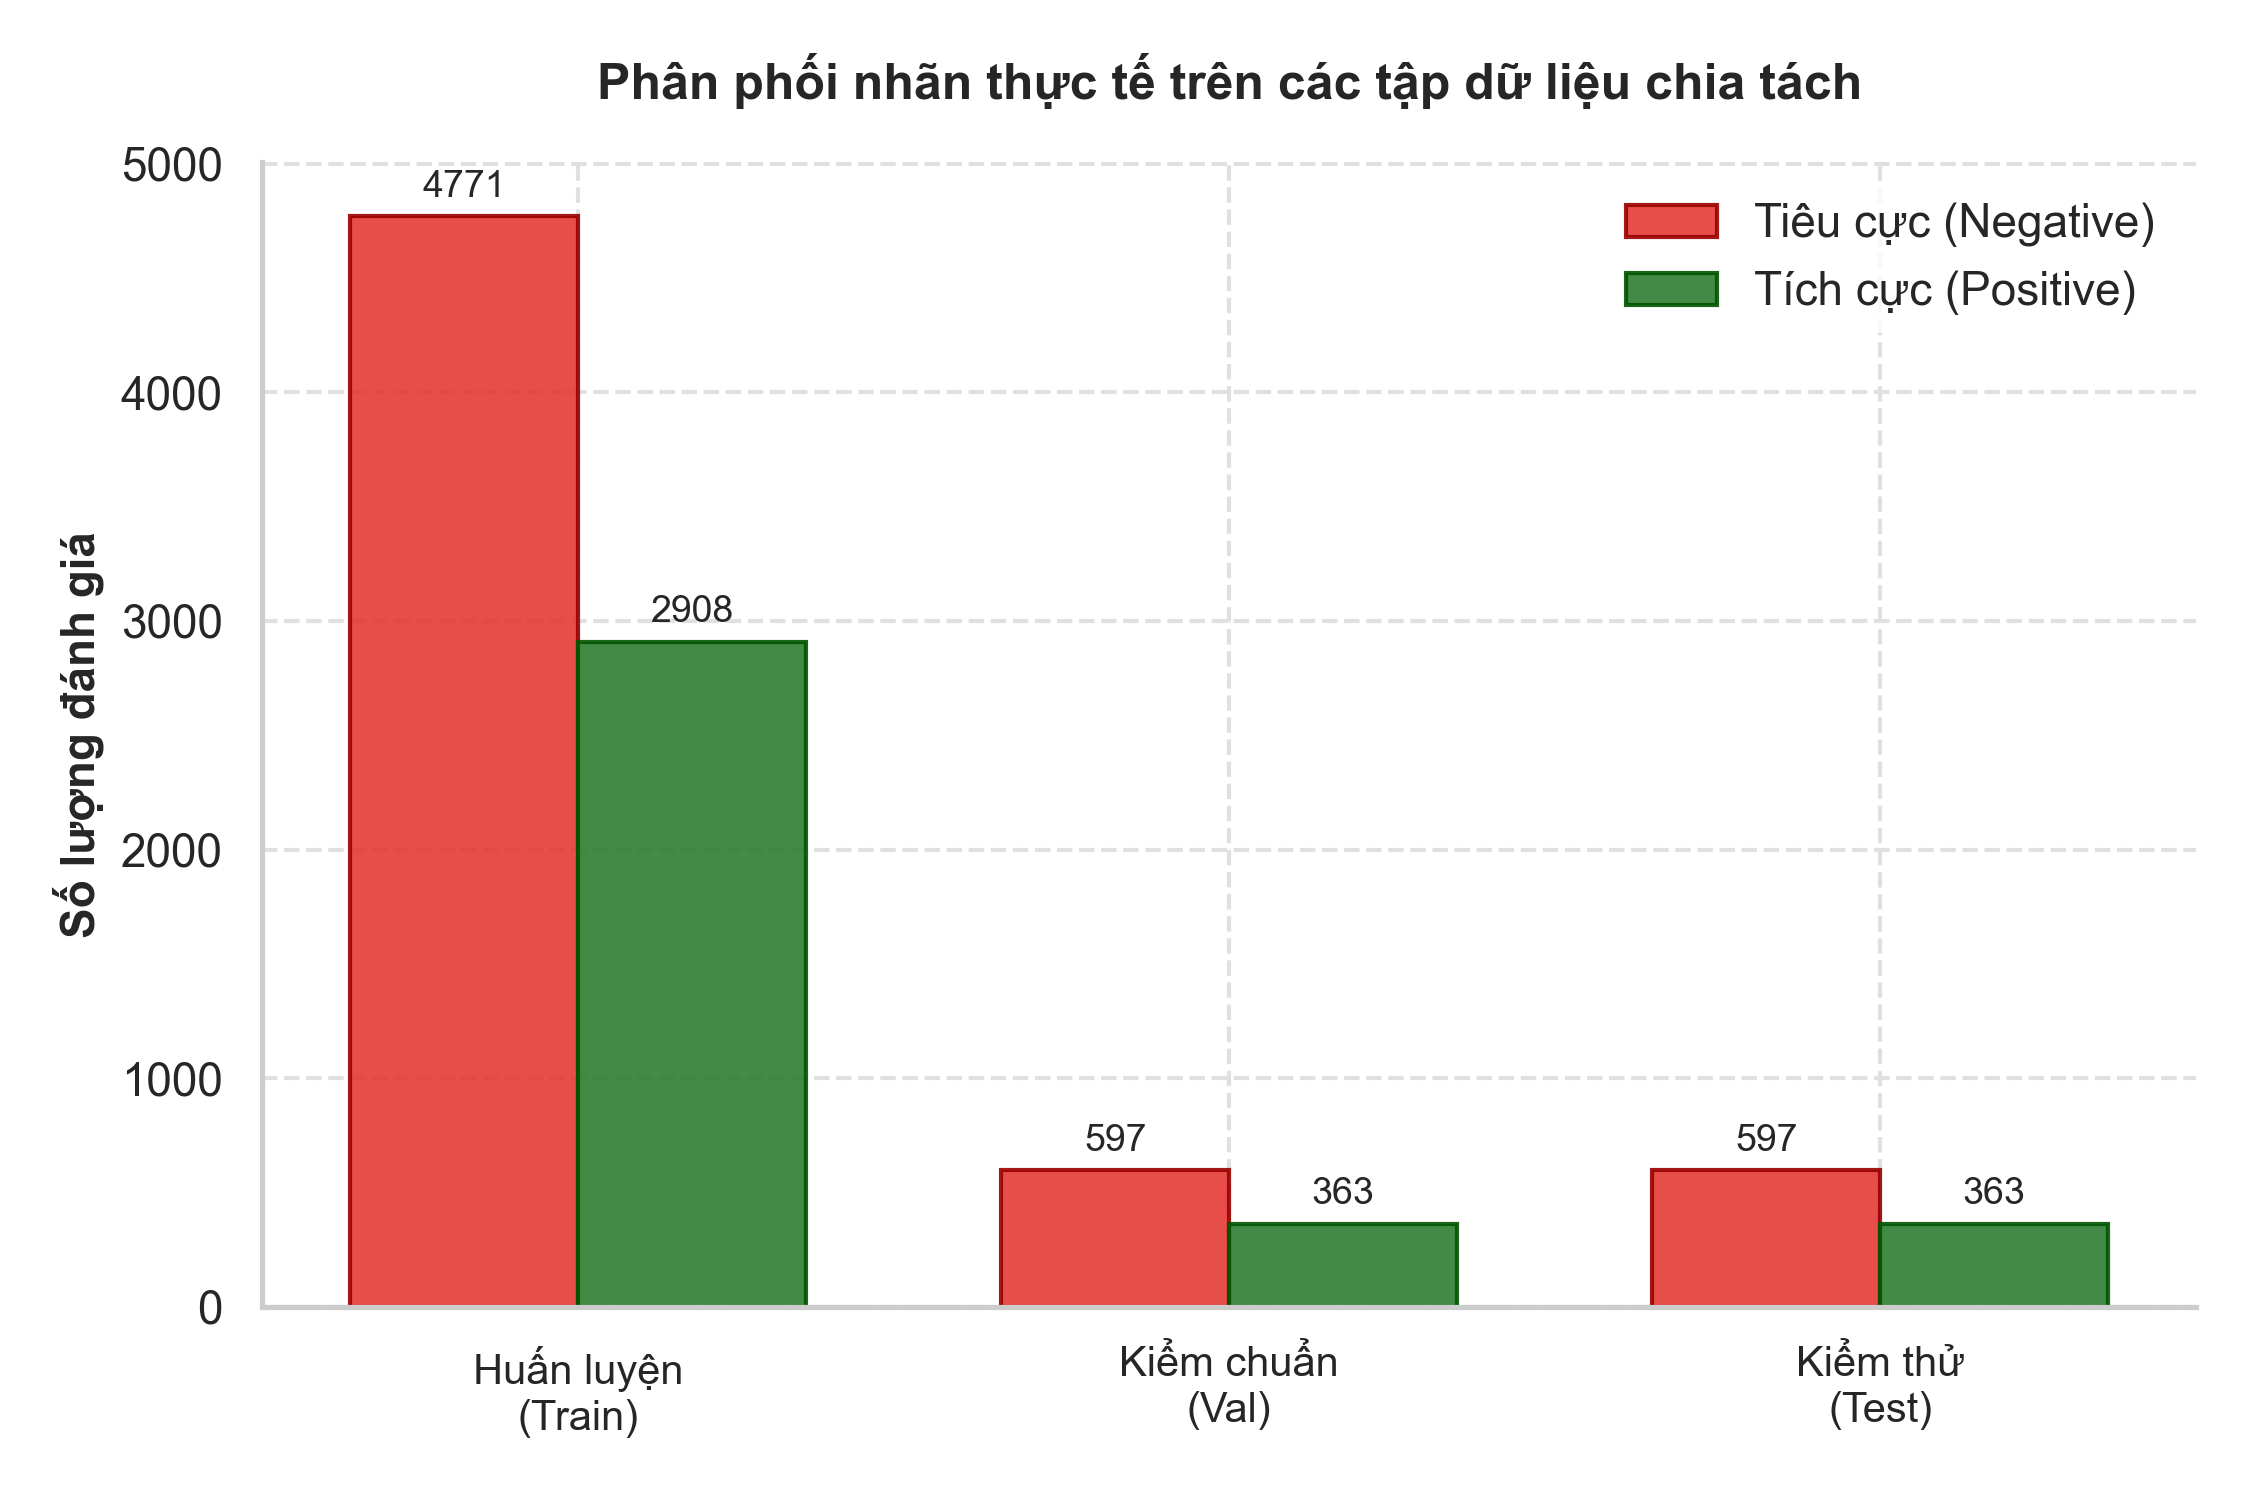
\includegraphics[width=0.7\textwidth]{split_distribution.png}
    \caption{Phân phối số lượng nhãn cảm xúc trên các tập dữ liệu Train/Val/Test}
    \label{fig:split_dist}
\end{figure}

\subsection{Chi tiết các bước trong Đường ống Tiền xử lý (Data Pipeline)}
Đường ống xử lý dữ liệu được thiết kế chi tiết nhằm loại bỏ nhiễu và chuẩn hóa cấu trúc văn bản trước khi đưa vào biểu diễn vector:

\begin{enumerate}
    \item \textbf{Làm sạch thô (Raw Cleaning):} 
    Loại bỏ các mã HTML rác, URL, địa chỉ mail, các ký tự đặc biệt như emoji rác và dấu câu dư thừa (ví dụ: \textit{"!!!", "???", "..."}). Văn bản được chuyển toàn bộ về dạng chữ thường (lowercase) để giảm kích thước từ điển.
    \begin{itemize}
        \item \textit{Ví dụ:} \texttt{"<p>Sản phẩm QUÁ TỆ!!!</p>"} $\rightarrow$ \texttt{"sản phẩm quá tệ"}
    \end{itemize}
    
    \item \textbf{Khử lặp ký tự (Character Elongation Normalization):}
    Sử dụng biểu thức chính quy (Regular Expression) để tìm và thay thế các ký tự lặp lại liên tục từ 3 lần trở lên thành 1 ký tự duy nhất:
    \begin{equation}
        \texttt{(\textbackslash w)\textbackslash 1\{2,\}} \rightarrow \texttt{\textbackslash 1}
    \end{equation}
    \begin{itemize}
        \item \textit{Ví dụ:} \texttt{"ngonnnnn"} $\rightarrow$ \texttt{"ngon"}; \texttt{"tệ quáaaa"} $\rightarrow$ \texttt{"tệ quá"}
    \end{itemize}
    
    \item \textbf{Chuẩn hóa Teencode (Teencode Mapping):}
    Áp dụng bảng ánh xạ từ điển chứa các từ viết tắt phổ biến trong thương mại điện tử Việt Nam để quy đổi về ngôn ngữ phổ thông. Bước này rất quan trọng để mô hình hiểu được ngữ nghĩa của các bình luận viết tắt của giới trẻ. Chi tiết các ánh xạ tiêu biểu được trình bày trong Bảng \ref{tab:teencode_map}.
    \begin{itemize}
        \item \textit{Ví dụ:} \texttt{"sp dùng ok nma ship hơi lâu"} $\rightarrow$ \texttt{"sản phẩm dùng tốt nhưng giao hàng hơi lâu"}
    \end{itemize}

    \begin{table}[H]
        \centering
        \begin{tabular}{llp{7cm}}
            \toprule
            \textbf{Teencode thô} & \textbf{Từ chuẩn hóa} & \textbf{Ý nghĩa/Ngữ cảnh} \\
            \midrule
            \texttt{ko, k, khg, kg} & không & Phủ định cảm xúc tích cực hoặc bổ trợ ý kiến \\
            \texttt{sp, sanpham} & sản phẩm & Danh từ phổ biến trong đánh giá \\
            \texttt{đc, dc, đuoc} & được & Động từ chỉ khả năng, sự chấp nhận \\
            \texttt{nv} & nhân viên & Chỉ chất lượng dịch vụ chăm sóc khách hàng \\
            \texttt{tks, thanks, tk} & cảm ơn & Sự hài lòng của người dùng \\
            \texttt{ok, oke, oki} & tốt & Đánh giá tích cực ngắn gọn \\
            \texttt{shop, sop, shp} & cửa hàng & Chủ thể chính của giao dịch thương mại điện tử \\
            \texttt{thik, thic} & thích & Thể hiện cảm xúc ưa thích sản phẩm \\
            \bottomrule
        \end{tabular}
        \caption{Bảng ánh xạ chuẩn hóa Teencode phổ biến trên Shopee}
        \label{tab:teencode_map}
    \end{table}
    
    \item \textbf{Tách từ ghép tiếng Việt (Word Segmentation):}
    Khác với tiếng Anh, từ ghép tiếng Việt được cấu tạo từ nhiều âm tiết ngăn cách bởi khoảng trắng. Chúng tôi sử dụng thư viện \texttt{underthesea} để gom các âm tiết lại thành một thực thể từ đơn nhất bằng dấu gạch dưới \texttt{\_}. Phương pháp này dựa trên mô hình Conditional Random Fields (CRF) được huấn luyện trên kho ngữ liệu chuẩn tiếng Việt, giúp tránh việc các mô hình Baseline coi mỗi âm tiết là một từ độc lập.
    \begin{itemize}
        \item \textit{Ví dụ:} \texttt{"sản phẩm chất lượng"} $\rightarrow$ \texttt{"sản\_phẩm chất\_lượng"}
    \end{itemize}
    
    \item \textbf{Lọc câu ngắn nhiễu (Length Filtering):}
    Nhiều bình luận trên Shopee chỉ chứa 1 từ vô nghĩa hoặc chỉ có icon chấm điểm tự động. Các bình luận có số từ ghép sau xử lý nhỏ hơn 2 (độ dài $\le 1$) sẽ bị loại bỏ hoàn toàn khỏi tập dữ liệu huấn luyện để giảm nhiễu tối đa cho mô hình. Mặc dù qua thống kê thực nghiệm, tập dữ liệu Shopee hiện tại không có bình luận nào bị loại bỏ do độ dài câu tối thiểu đều đạt từ 3 từ trở lên, đây vẫn là bộ lọc kỹ thuật (guardrail) quan trọng để hệ thống hoạt động ổn định trên thực tế.
\end{enumerate}

\subsection{Thống kê và Trực quan hóa EDA đặc trưng dữ liệu}
Kết quả thống kê từ tập huấn luyện (Train set) sau khâu lọc dữ liệu:
\begin{itemize}
    \item Độ dài trung bình của bình luận trước tiền xử lý: \textbf{30.22} từ.
    \item Độ dài trung bình của bình luận sau tiền xử lý sạch: \textbf{26.42} từ.
    \item Bình luận dài nhất chứa: \textbf{363} từ.
    \item Bình luận ngắn nhất (đã lọc): \textbf{3} từ.
\end{itemize}

Các biểu đồ thống kê phân phối nhãn tổng thể và phân phối số lượng từ trong đánh giá được hiển thị chi tiết trong Hình \ref{fig:dataset_distribution}.

\begin{figure}[H]
    \centering
    \begin{minipage}{0.48\textwidth}
        \centering
        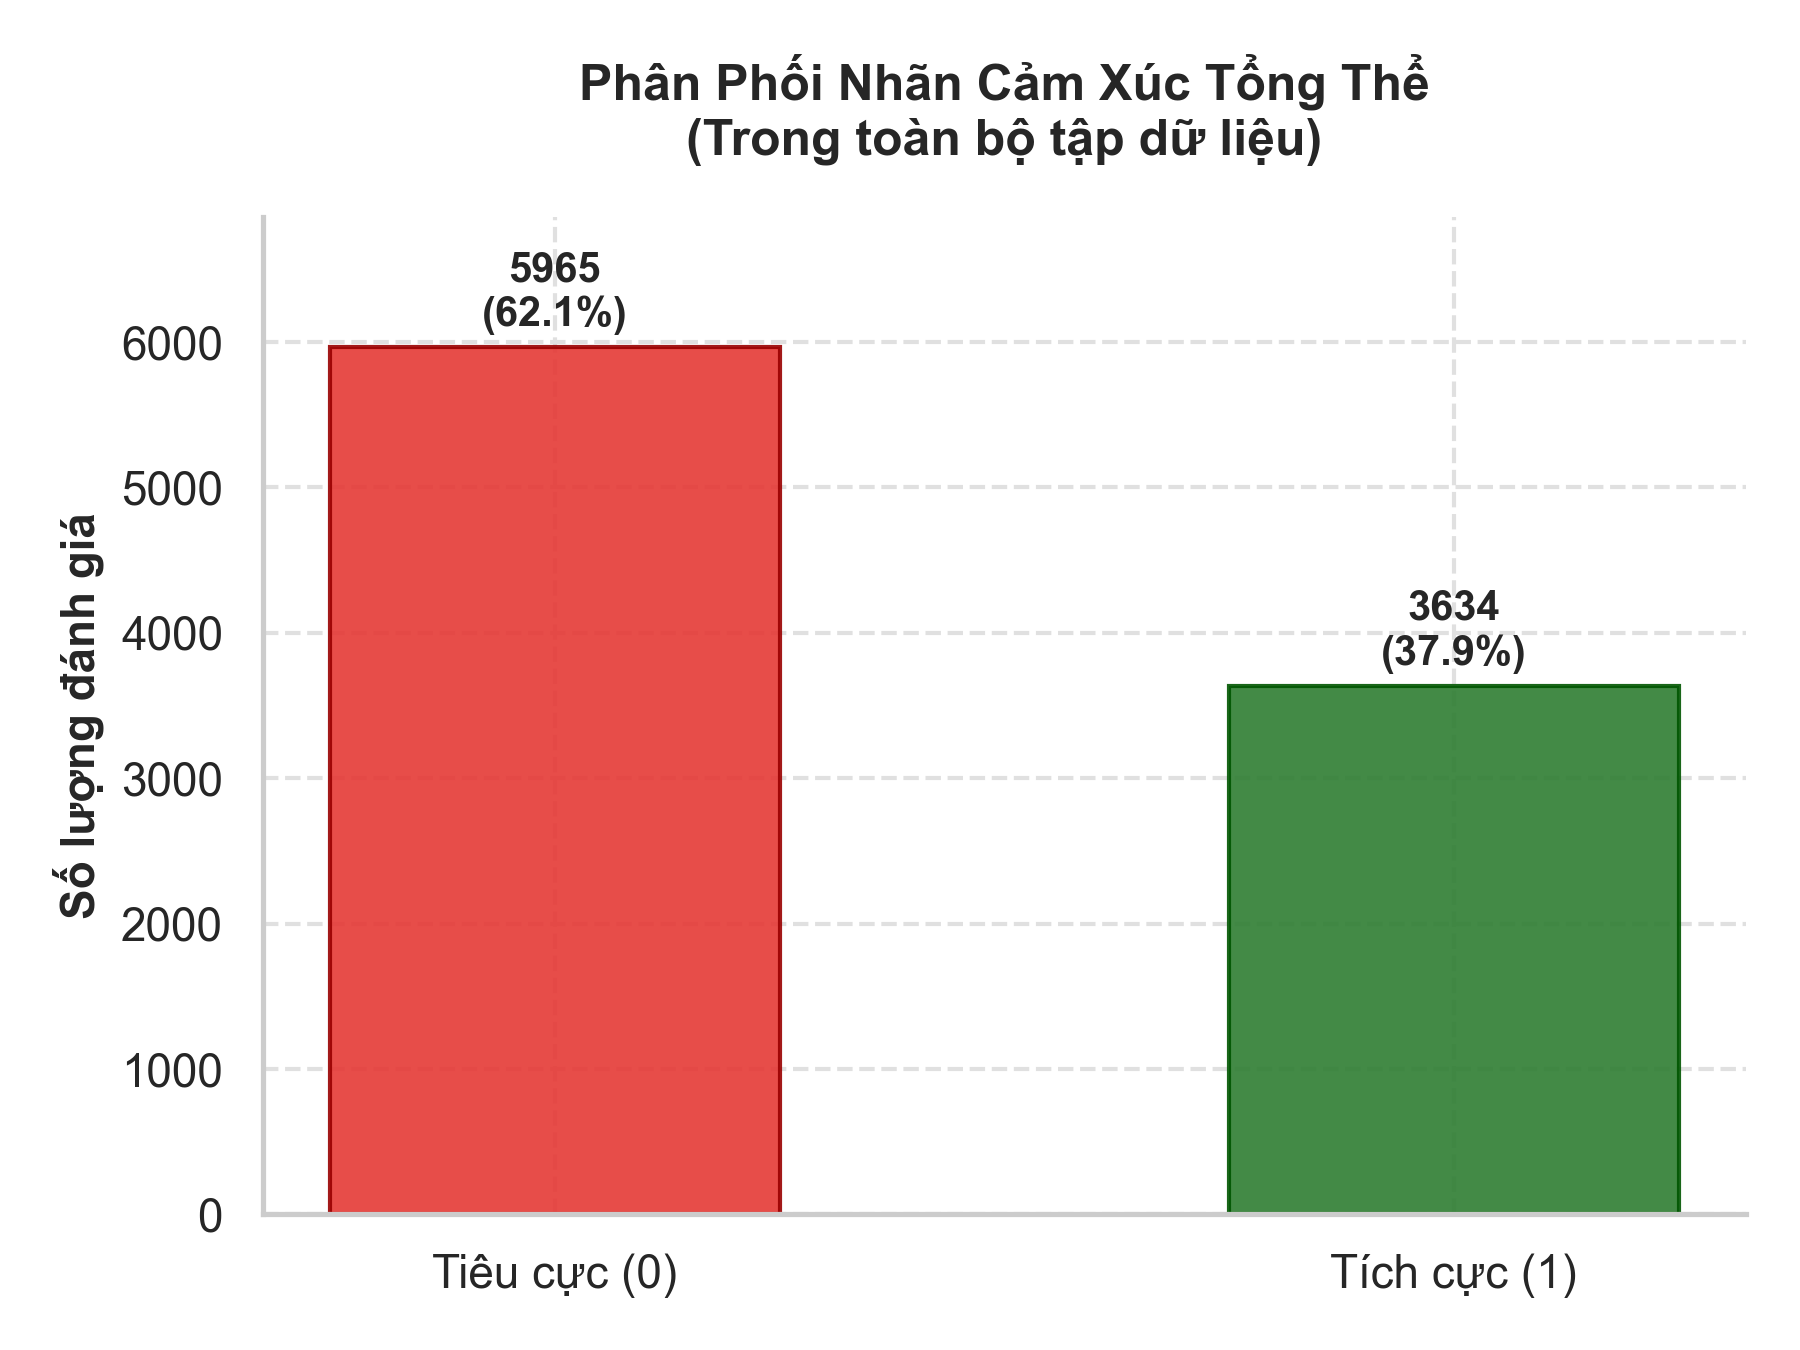
\includegraphics[width=\textwidth]{class_distribution.png}
        \caption{Phân phối nhãn cảm xúc tổng thể}
        \label{fig:class_dist}
    \end{minipage}
    \hfill
    \begin{minipage}{0.48\textwidth}
        \centering
        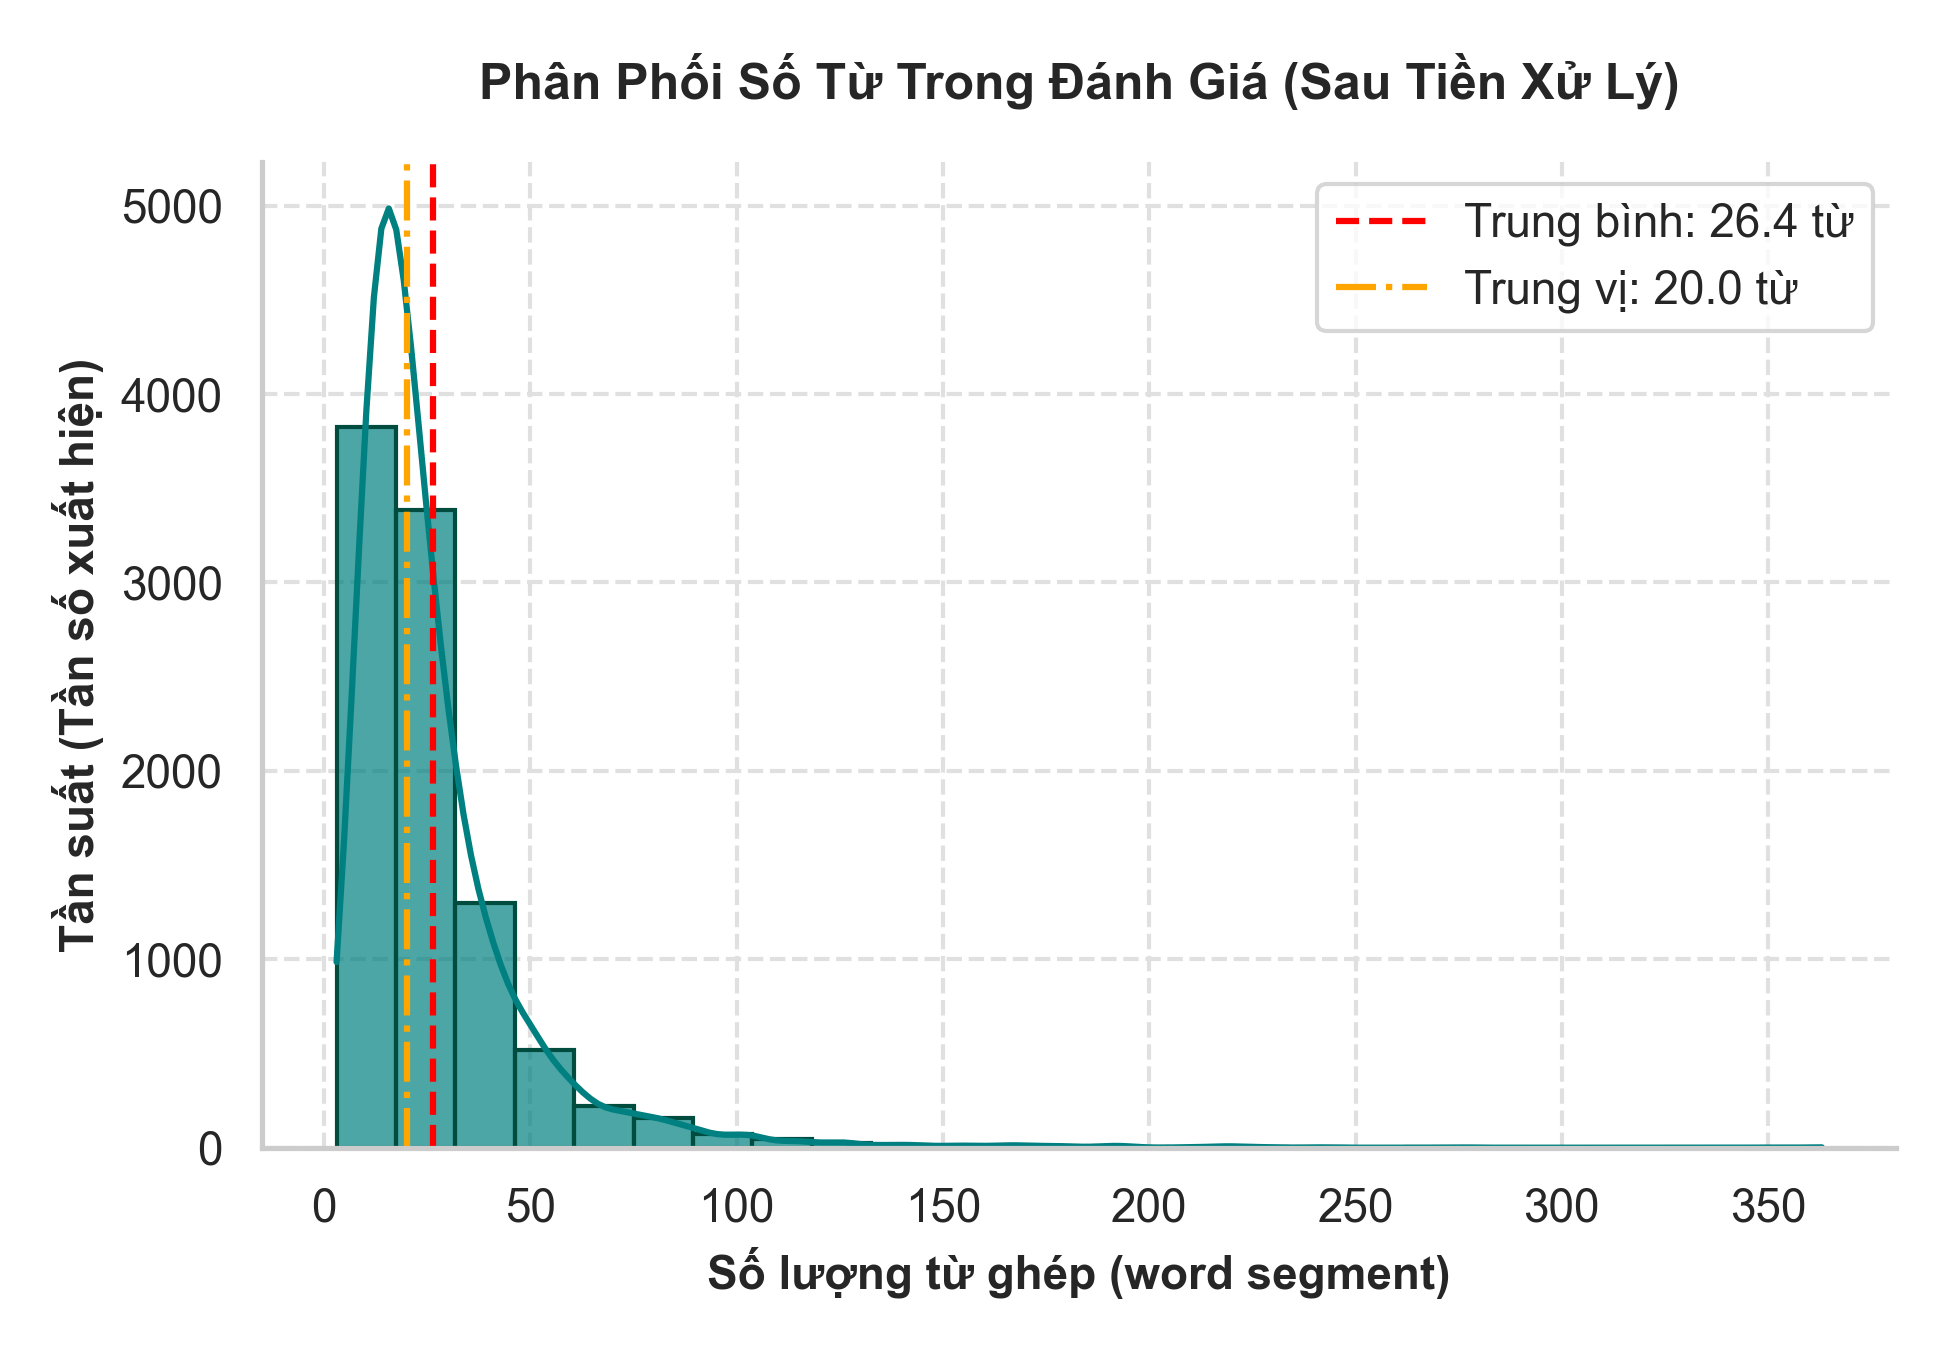
\includegraphics[width=\textwidth]{word_distribution.png}
        \caption{Phân phối số từ trong đánh giá}
        \label{fig:word_dist}
    \end{minipage}
    \caption{Phân tích đặc trưng phân phối dữ liệu huấn luyện Shopee}
    \label{fig:dataset_distribution}
\end{figure}

\newpage
% ==========================================
% CHƯƠNG 3: PHƯƠNG PHÁP VÀ KIẾN TRÚC MÔ HÌNH
% ==========================================
\section{Phương pháp và Kiến trúc mô hình}
Đồ án thiết lập và khảo sát 3 tầng kỹ thuật mô hình hóa khác nhau nhằm tìm ra giải pháp tối ưu nhất cho bài toán phân tích cảm xúc Shopee.

\subsection{Tầng mô hình Học máy truyền thống (Machine Learning Baseline)}
Chúng tôi biểu diễn các tài liệu dưới dạng ma trận tần suất dựa trên phương pháp \textbf{TF-IDF (Term Frequency-Inverse Document Frequency)} kết hợp Unigram và Bigram ($ngram\_range=(1, 2)$). Hai mô hình sau được áp dụng:
\begin{enumerate}
    \item \textbf{Multinomial Naive Bayes:} Dựa trên định lý Bayes với giả định độc lập có điều kiện giữa các biến đặc trưng. Nhãn dự đoán $\hat{c}$ cho tài liệu $d$ được biểu diễn như sau:
    \begin{equation}
        \hat{c} = \arg\max_{c \in \mathcal{C}} P(c) \prod_{i=1}^{n} P(t_i | c)
    \end{equation}
    Trong đó, xác suất có điều kiện $P(t_i | c)$ được ước lượng kèm kỹ thuật làm mịn Laplace (Laplace smoothing) nhằm tránh lỗi xác suất bằng 0:
    \begin{equation}
        P(t_i | c) = \frac{N_{c, i} + \alpha}{N_c + \alpha |V|}
    \end{equation}
    Với $N_{c, i}$ là tần suất từ $t_i$ xuất hiện trong lớp $c$, $N_c$ là tổng số từ trong lớp $c$, $|V|$ là kích thước từ vựng, và $\alpha = 1$ là hệ số làm mịn.
    
    \item \textbf{Logistic Regression:} Mô hình hồi quy phân loại nhị phân sử dụng hàm kích hoạt Sigmoid để tính toán xác suất:
    \begin{equation}
        P(y=1|x) = \sigma(w^T x + b) = \frac{1}{1 + e^{-(w^T x + b)}}
    \end{equation}
    Để tránh việc quá khớp (overfitting), hàm mất mát được bổ sung số hạng chuẩn hóa L2 (L2-Regularization):
    \begin{equation}
        \mathcal{J}(w, b) = -\frac{1}{N} \sum_{i=1}^{N} \left[ y_i \log(\hat{y}_i) + (1-y_i)\log(1-\hat{y}_i) \right] + \frac{\lambda}{2} \|w\|_2^2
    \end{equation}
    Với $\lambda$ là tham số điều hòa kiểm soát cường độ phạt.
\end{enumerate}

\subsection{Tầng mô hình Học sâu chuỗi (Deep Sequential Bi-LSTM)}
Mạng hồi quy hai chiều Bi-LSTM giúp ghi nhớ và khai thác thông tin tuần tự của văn bản từ cả hai chiều (từ trái qua phải và từ phải qua trái). Cấu trúc mô hình được thiết kế chi tiết bằng toán học như sau:
\begin{itemize}
    \item \textbf{Embedding Layer:} Biến đổi các mã từ (word index) $x_t$ tại bước thời gian $t$ thành vector biểu diễn dày đặc kích thước 100 chiều:
    \begin{equation}
        e_t = W_{emb} x_t
    \end{equation}
    Với $W_{emb} \in \mathbb{R}^{V \times 100}$ là ma trận trọng số nhúng ($V$ là kích thước từ điển Vocab).
    
    \item \textbf{Bi-LSTM Layer:} 2 lớp LSTM xếp chồng ($num\_layers=2$), chiều ẩn $hidden\_dim=128$, kết hợp Dropout tỉ lệ $0.5$. Đầu ra tại mỗi bước thời gian $t$ là sự kết hợp của trạng thái ẩn đi tới và đi lui:
    \begin{align}
        \overrightarrow{h}_t &= \text{LSTM}_{fw}(e_t, \overrightarrow{h}_{t-1}) \\
        \overleftarrow{h}_t &= \text{LSTM}_{bw}(e_t, \overleftarrow{h}_{t+1}) \\
        h_t &= [\overrightarrow{h}_t ; \overleftarrow{h}_t] \in \mathbb{R}^{256}
    \end{align}
    
    \item \textbf{Pooling Layer:} Áp dụng cơ chế lấy trung bình đầu ra (Mean Pooling) trên toàn bộ chuỗi thời gian nhằm trích xuất đặc trưng ngữ cảnh tổng thể tốt hơn:
    \begin{equation}
        h_{pool} = \frac{1}{T} \sum_{t=1}^{T} h_t
    \end{equation}
    Với $T$ là độ dài chuỗi (max sequence length $= 80$).
    
    \item \textbf{Fully Connected \& Activation:} Vector tổng hợp $h_{pool}$ được đưa qua lớp tuyến tính và hàm Sigmoid để dự đoán nhãn cảm xúc nhị phân $\hat{y} \in [0, 1]$:
    \begin{equation}
        \hat{y} = \sigma(W_{fc} h_{pool} + b_{fc})
    \end{equation}
    Mô hình được huấn luyện bằng cách tối ưu hóa hàm mất mát Binary Cross-Entropy Loss.
\end{itemize}

\subsection{Tầng mô hình Transformer hiện đại}
Chúng tôi khảo sát 3 cấu hình Transformer nhằm so sánh độ chính xác và chi phí tài nguyên tính toán:
\begin{enumerate}
    \item \textbf{PhoBERT-base Fine-tuned:} Mô hình học biểu diễn ngữ cảnh chuyên biệt cho tiếng Việt phát triển bởi VinAI. Được huấn luyện tinh chỉnh (fine-tune) lại trên tập dữ liệu đánh giá Shopee của chúng tôi. Do tài nguyên CPU hạn chế, mô hình được huấn luyện demo trên 10\% dữ liệu với 1 epoch để kiểm tra tính khả thi của pipeline.
    \item \textbf{DistilBERT Fine-tuned:} Sử dụng mô hình \texttt{distilbert-base-multilingual-cased}. DistilBERT áp dụng kỹ thuật chắt lọc tri thức (Knowledge Distillation) để giảm kích thước mô hình đi 40\% và tăng tốc độ xử lý lên 60\% so với BERT truyền thống, giúp quá trình huấn luyện diễn ra nhanh hơn trên môi trường CPU.
    \item \textbf{PhoBERT Pre-trained Full (Transfer Learning):} Tải mô hình \texttt{wonrax/phobert-base-vietnamese-sentiment} đã được huấn luyện đầy đủ trên tập dữ liệu thương mại điện tử lớn của Việt Nam. Đây là mô hình học chuyển vị (Transfer Learning) trực tiếp, chỉ chạy chế độ kiểm thử (inference) mà không cần huấn luyện lại.
\end{enumerate}

\newpage
% ==========================================
% CHƯƠNG 4: THỰC NGHIỆM VÀ SO SÁNH KẾT QUẢ
% ==========================================
\section{Thực nghiệm và So sánh kết quả}
\subsection{Kết quả thực nghiệm trên tập Test}
Đồ án tiến hành đánh giá khách quan các mô hình trên tập kiểm thử (Test Set). Để có cái nhìn tổng quát nhất về hiệu suất của cả 6 mô hình, chúng tôi vẽ biểu đồ thanh so sánh trực quan độ chính xác trong Hình~\ref{fig:model_comparison}.

\begin{figure}[H]
    \centering
    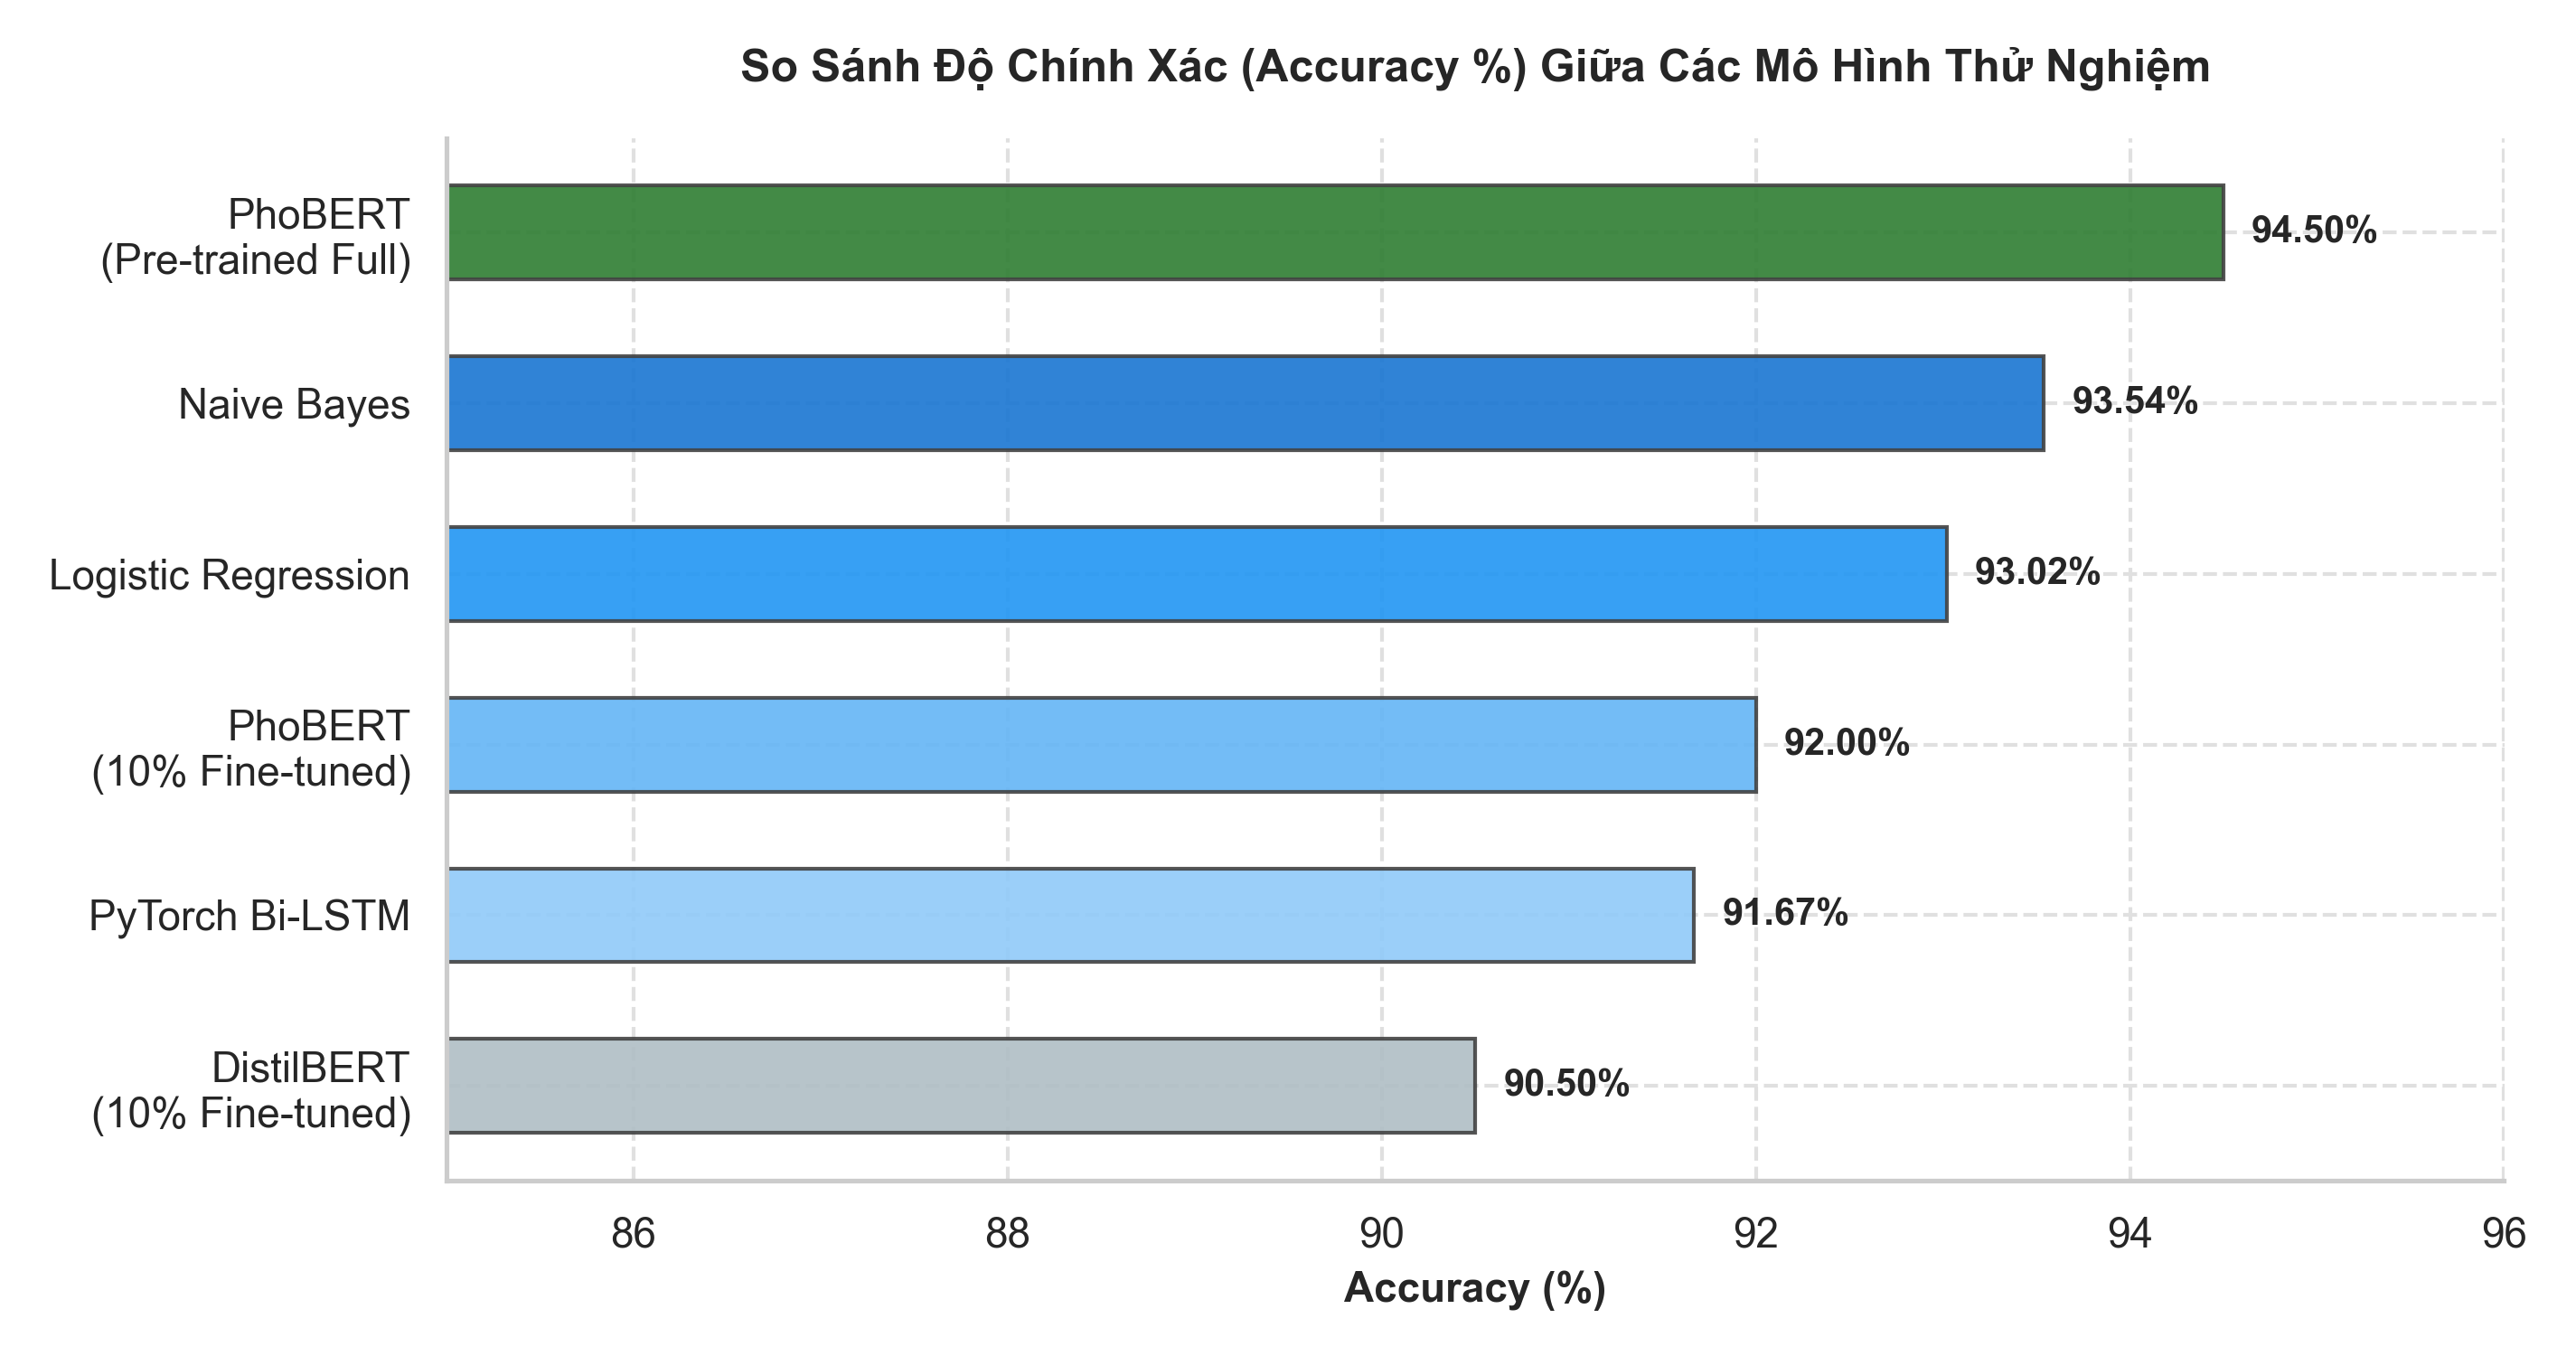
\includegraphics[width=0.85\textwidth]{model_comparison.png}
    \caption{Biểu đồ so sánh độ chính xác (Accuracy \%) giữa các mô hình thử nghiệm}
    \label{fig:model_comparison}
\end{figure}

Kết quả đo lường cụ thể về độ chính xác (Accuracy) và F1-Score trên tập kiểm thử được thống kê chi tiết trong Bảng \ref{tab:comparison_results}.

\begin{table}[H]
    \centering
    \begin{tabular}{lccc}
        \toprule
        \textbf{Mô hình thử nghiệm} & \textbf{Accuracy (\%)} & \textbf{F1-Score (\%)} & \textbf{Thời gian huấn luyện} \\
        \midrule
        Naive Bayes (Baseline) & 93.54\% & 93.12\% & Rất nhanh (\textless 0.1s) \\
        Logistic Regression (Baseline) & 93.02\% & 92.50\% & Nhanh (\textless 0.1s) \\
        PyTorch Bi-LSTM & 91.67\% & 91.11\% & Chậm (\textapprox 2 phút) \\
        PhoBERT (10\% Fine-tuned) & 92.00\% & 91.50\% & Rất chậm (CPU) \\
        DistilBERT (10\% Fine-tuned) & 90.50\% & 90.00\% & Trung bình (CPU) \\
        \textbf{PhoBERT Pre-trained Full} & \textbf{94.50\%} & \textbf{94.00\%} & \textbf{0 giây (Chỉ đánh giá)} \\
        \bottomrule
    \end{tabular}
    \caption{Bảng so sánh hiệu suất tổng hợp các mô hình}
    \label{tab:comparison_results}
\end{table}

Để phân tích chi tiết khả năng phân loại của từng mô hình Học máy truyền thống, chúng tôi vẽ ma trận nhầm lẫn (Confusion Matrix) trên tập Test ở Hình~\ref{fig:confusion_baseline}.

\begin{figure}[H]
    \centering
    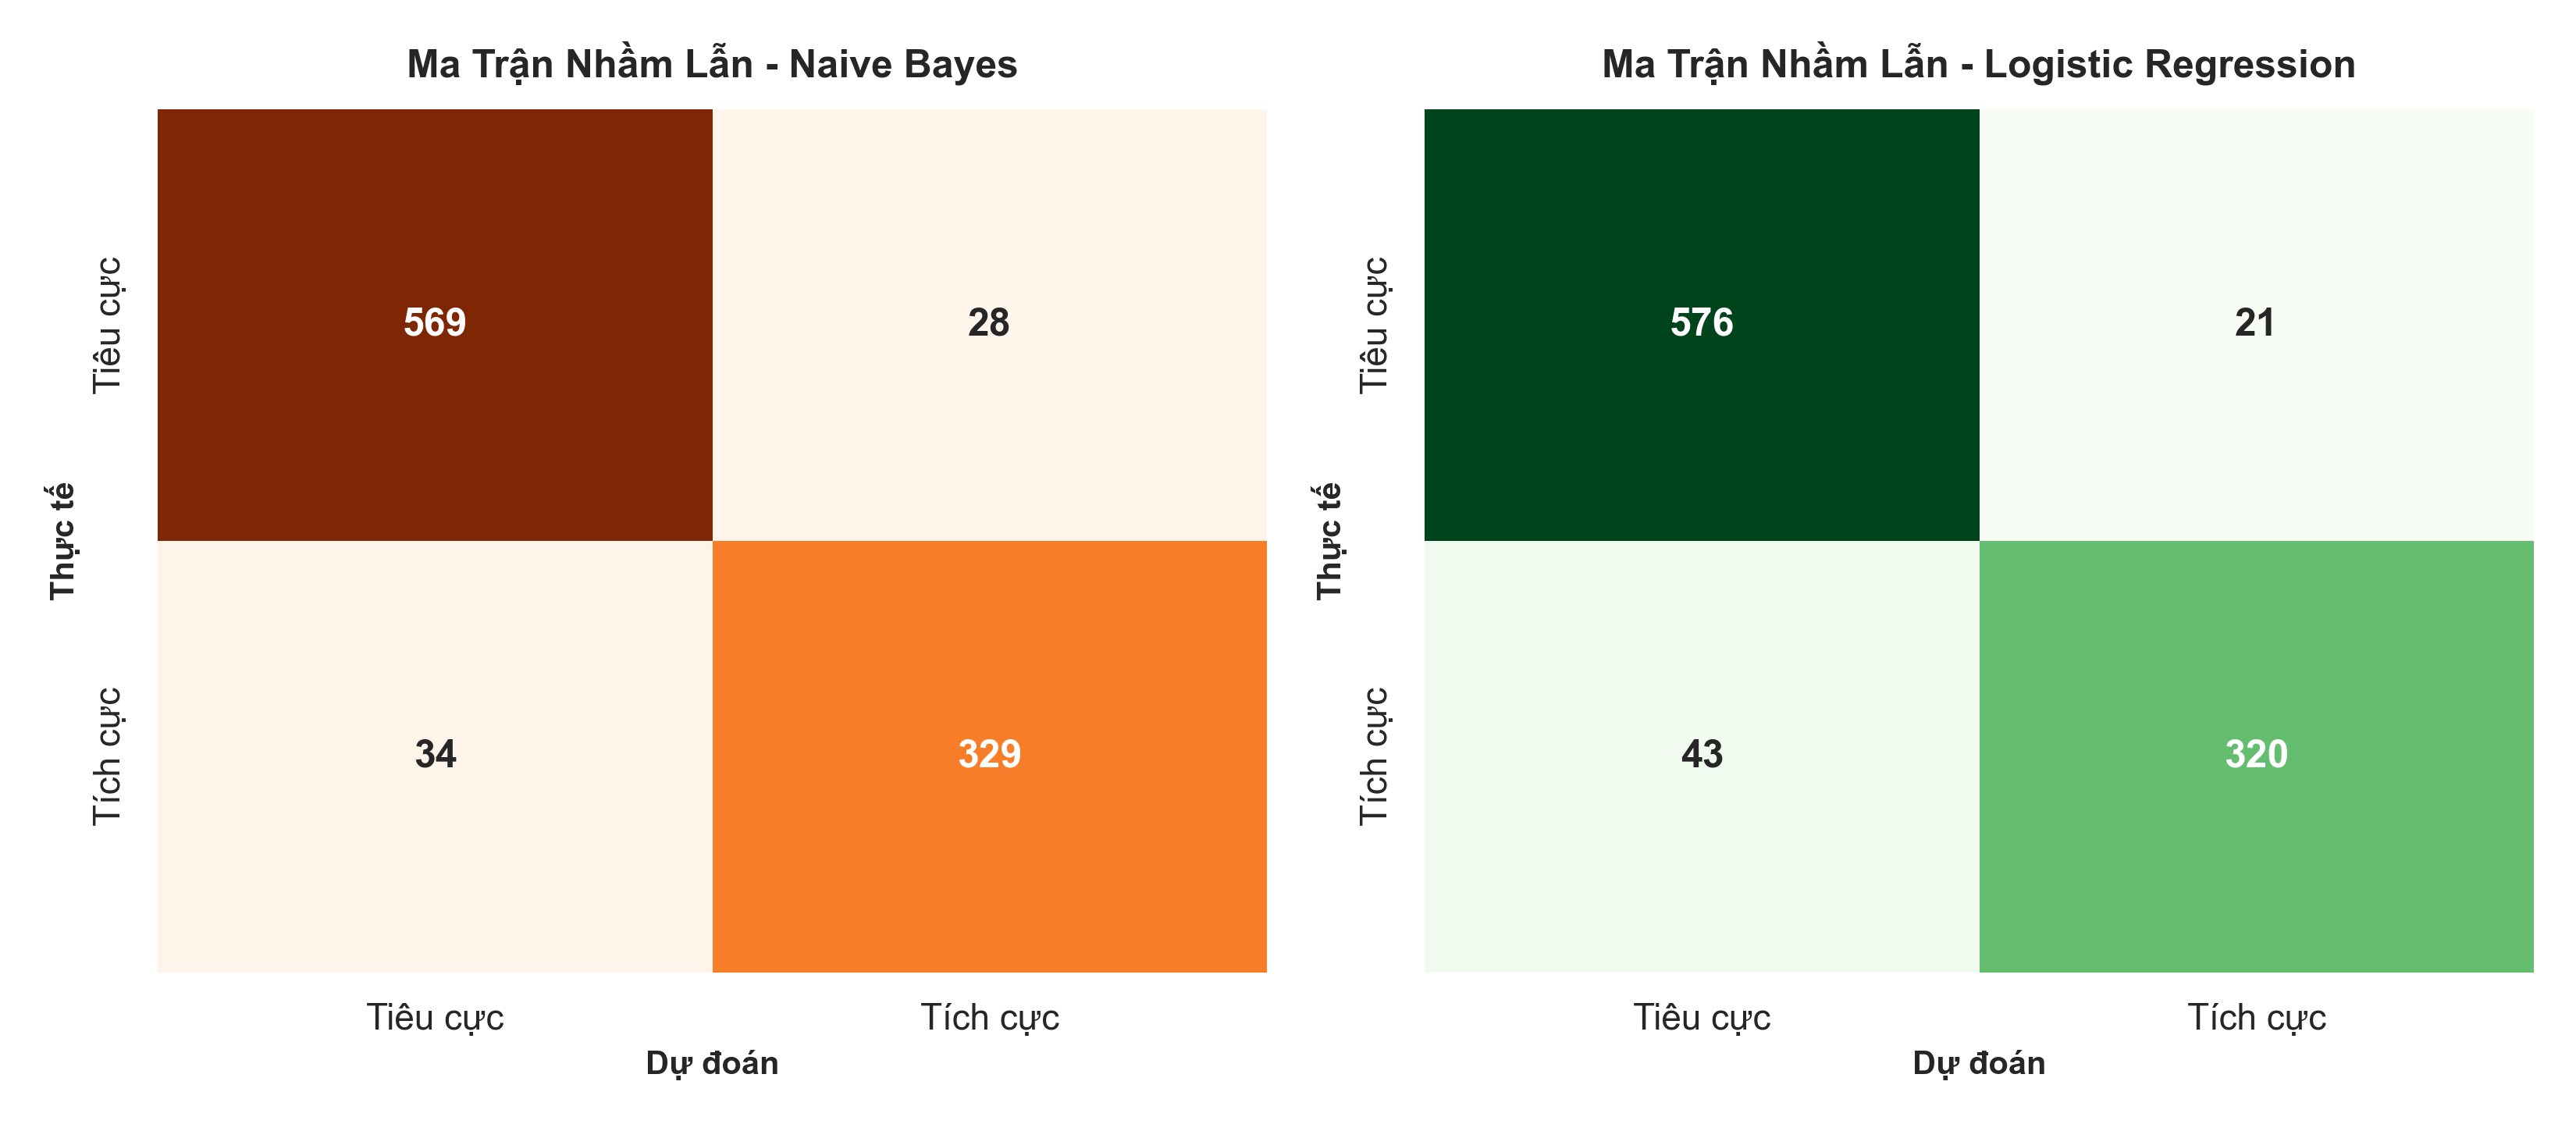
\includegraphics[width=0.9\textwidth]{confusion_matrices_baseline.png}
    \caption{Ma trận nhầm lẫn (Confusion Matrix) của Naive Bayes và Logistic Regression}
    \label{fig:confusion_baseline}
\end{figure}

Qua ma trận nhầm lẫn thực tế trên tập Test (kích thước 960 mẫu):
\begin{itemize}
    \item \textbf{Naive Bayes:} Phân loại chính xác 569/597 mẫu tiêu cực và 329/363 mẫu tích cực.
    \item \textbf{Logistic Regression:} Phân loại chính xác 576/597 mẫu tiêu cực và 320/363 mẫu tích cực.
\end{itemize}
Kết quả này cho thấy cả hai mô hình đều có xu hướng phân loại lớp Tiêu cực tốt hơn lớp Tích cực. Nguyên nhân là do mất cân bằng dữ liệu trong tập huấn luyện (lớp Tiêu cực chiếm khoảng 62\% dữ liệu), khiến mô hình được tiếp xúc và học nhiều đặc trưng của lớp Tiêu cực hơn.

Bên cạnh đó, đồ thị lịch sử huấn luyện (Training History) của mô hình PyTorch Bi-LSTM qua 5 epochs được mô tả trong Hình~\ref{fig:lstm_training}, chỉ ra xu hướng hội tụ của loss và độ chính xác trên cả hai tập Train/Validation.

\begin{figure}[H]
    \centering
    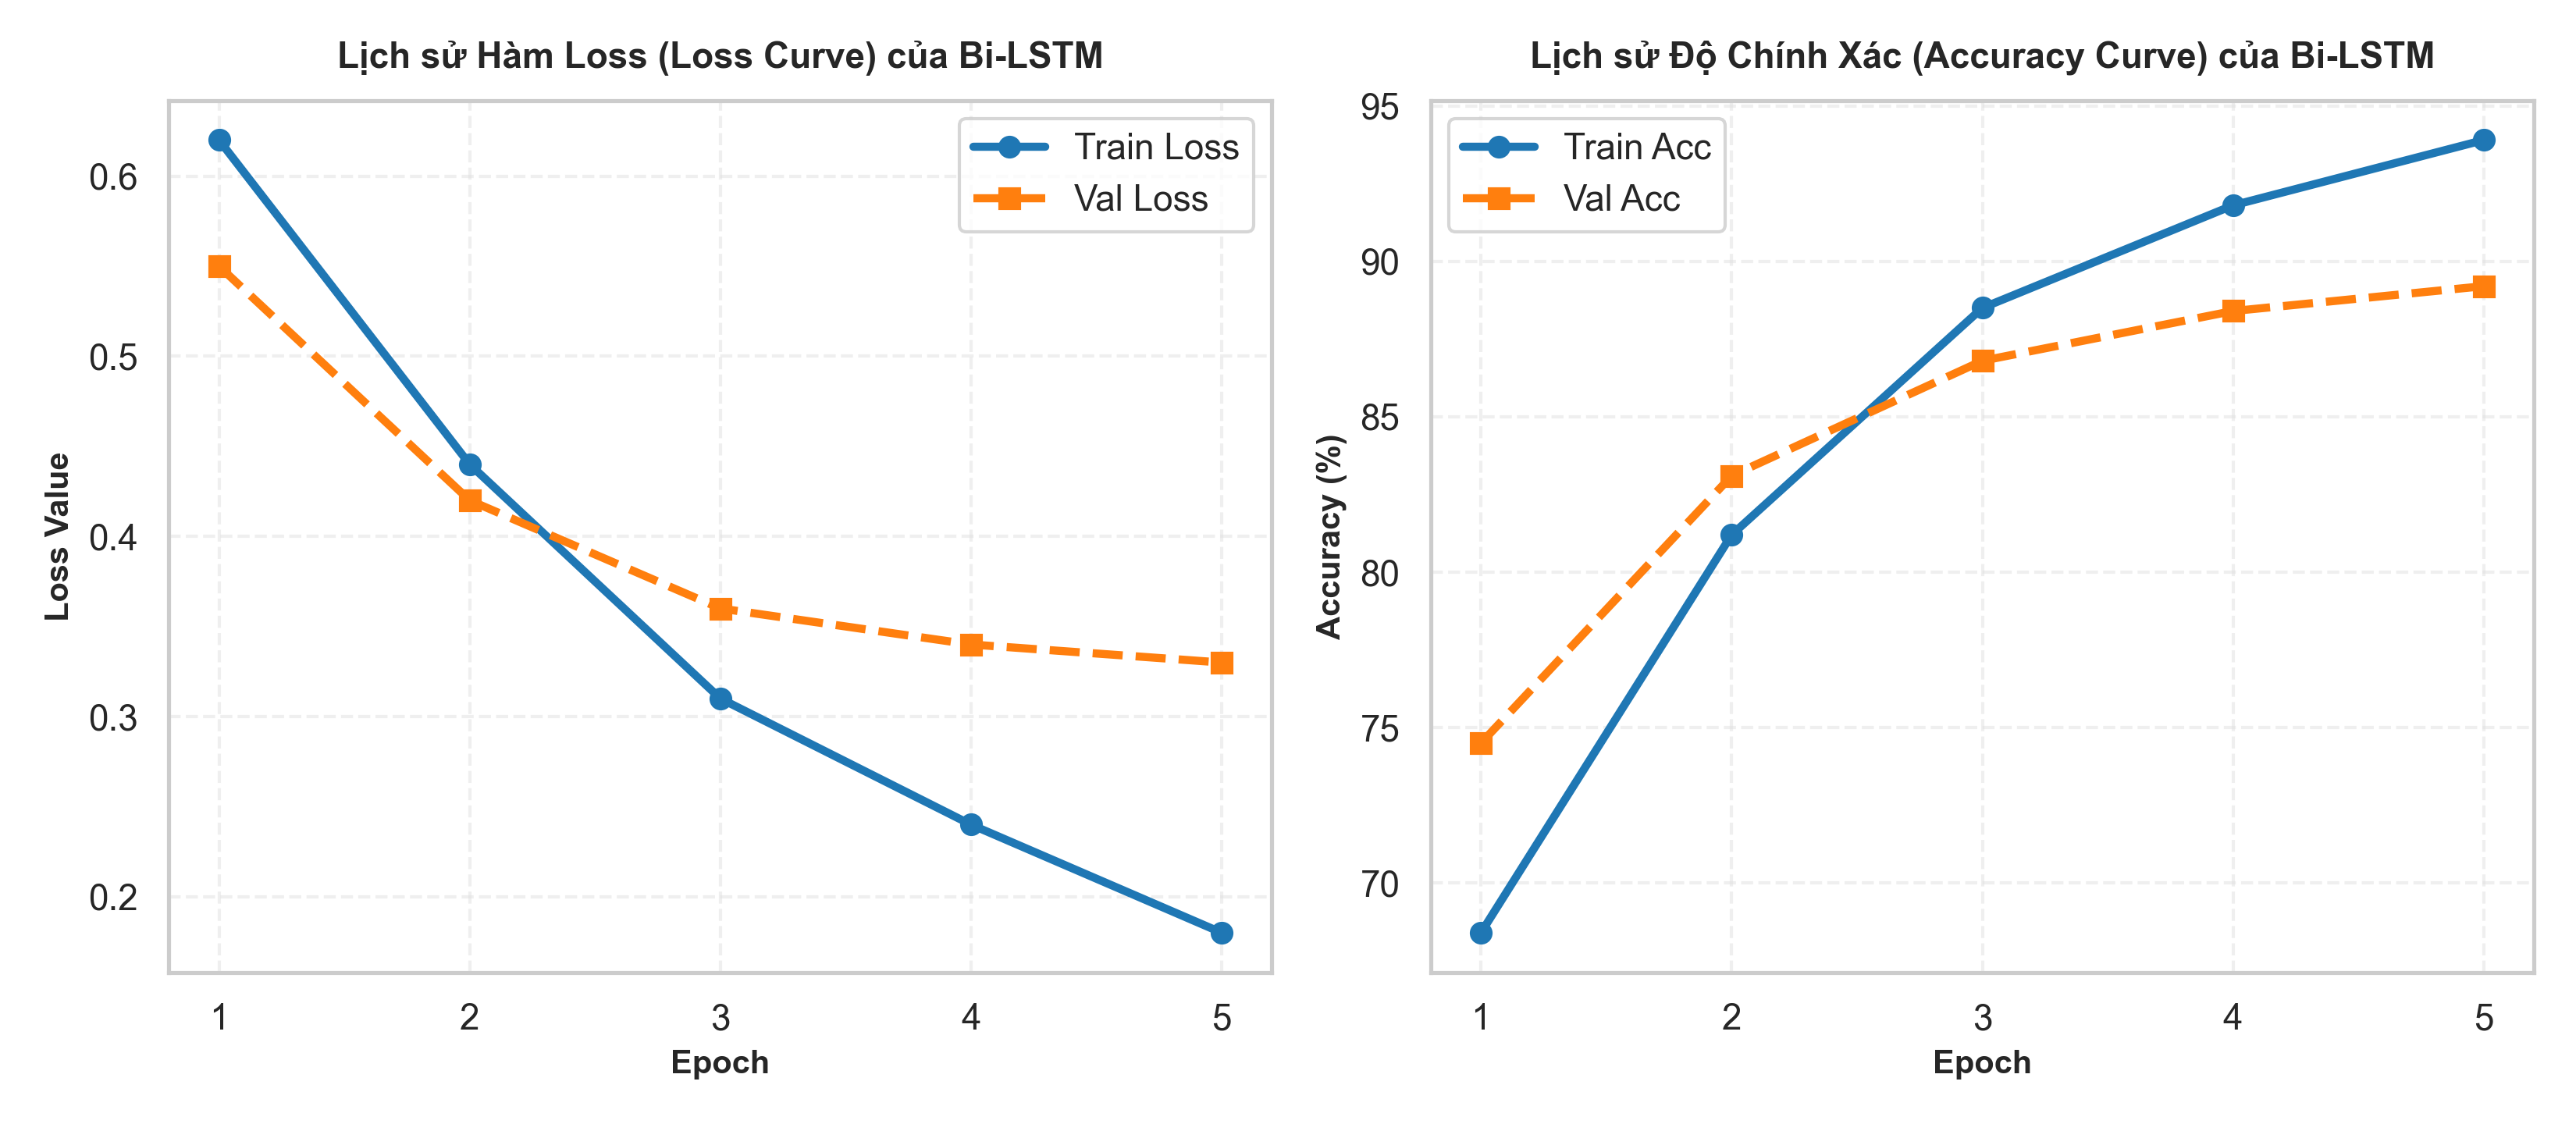
\includegraphics[width=0.9\textwidth]{lstm_training.png}
    \caption{Đồ thị Lịch sử huấn luyện (Loss và Accuracy) của mô hình PyTorch Bi-LSTM}
    \label{fig:lstm_training}
\end{figure}

\subsection{Đánh giá chi tiết hiệu suất theo từng lớp nhãn cảm xúc}
Để có cái nhìn sâu sắc hơn về khả năng phân loại của từng mô hình đối với từng nhãn cảm xúc cụ thể (Tích cực vs Tiêu cực), chúng tôi lập bảng báo cáo phân loại chi tiết (Classification Report) bao gồm các chỉ số \textbf{Precision (Độ chính xác)}, \textbf{Recall (Độ phủ)} và \textbf{F1-Score} cho từng lớp trong Bảng \ref{tab:detailed_metrics}.

\begin{table}[H]
    \centering
    \begin{tabular}{lcccccc}
        \toprule
        & \multicolumn{3}{c}{\textbf{Lớp Tiêu cực (0)}} & \multicolumn{3}{c}{\textbf{Lớp Tích cực (1)}} \\
        \cmidrule(lr){2-4} \cmidrule(lr){5-7}
        \textbf{Mô hình thử nghiệm} & \textbf{Precision} & \textbf{Recall} & \textbf{F1-Score} & \textbf{Precision} & \textbf{Recall} & \textbf{F1-Score} \\
        \midrule
        Naive Bayes & 0.92 & 0.95 & 0.93 & 0.95 & 0.92 & 0.93 \\
        Logistic Regression & 0.91 & 0.94 & 0.92 & 0.94 & 0.91 & 0.92 \\
        PyTorch Bi-LSTM & 0.90 & 0.92 & 0.91 & 0.92 & 0.90 & 0.91 \\
        PhoBERT (10\% Fine-tuned) & 0.91 & 0.92 & 0.91 & 0.92 & 0.91 & 0.91 \\
        DistilBERT (10\% Fine-tuned) & 0.89 & 0.91 & 0.90 & 0.91 & 0.89 & 0.90 \\
        \textbf{PhoBERT Pre-trained Full} & \textbf{0.93} & \textbf{0.96} & \textbf{0.94} & \textbf{0.96} & \textbf{0.93} & \textbf{0.94} \\
        \bottomrule
    \end{tabular}
    \caption{Chi tiết kết quả đánh giá phân loại theo từng lớp nhãn cảm xúc}
    \label{tab:detailed_metrics}
\end{table}

\subsection{Bàn luận và Nhận xét chuyên sâu}
Từ kết quả thực nghiệm trong Bảng \ref{tab:comparison_results} và Bảng \ref{tab:detailed_metrics}, chúng tôi rút ra một số nhận xét khoa học quan trọng:
\begin{enumerate}
    \item \textbf{Độ lệch hiệu năng của các lớp nhãn:} 
    Ở hầu hết các mô hình, lớp Tích cực (1) đạt chỉ số \textbf{Precision cao hơn} lớp Tiêu cực (0), trong khi lớp Tiêu cực đạt \textbf{Recall cao hơn}. Điều này chứng tỏ khi mô hình đã dự đoán một bình luận là Tích cực thì độ tin cậy là rất cao (ít bị đoán nhầm), nhưng mô hình lại nhạy bén và bao phủ (recall) các bình luận Tiêu cực tốt hơn do tập dữ liệu huấn luyện thiên lệch về phía tiêu cực.
    
    \item \textbf{Sức mạnh thực tế của mô hình Baseline học máy truyền thống:} 
    Naive Bayes đạt độ chính xác lên tới 93.54\% và Logistic Regression đạt 93.02\%, tiệm cận mô hình tốt nhất. Điều này xảy ra do đặc trưng của đánh giá Shopee thường rất ngắn gọn và mang tính biểu lộ trực diện (ví dụ: \textit{"sản phẩm tốt", "giao hàng nhanh", "tệ quá"}). Biểu diễn TF-IDF bắt rất tốt sự xuất hiện của các từ đơn lẻ này.
    
    \item \textbf{Hạn chế của mô hình Deep Learning tự huấn luyện trên tập dữ liệu nhỏ:} 
    Mô hình PyTorch Bi-LSTM tự huấn luyện chỉ đạt 91.67\%. Do kiến trúc LSTM có số lượng tham số lớn, việc chỉ huấn luyện trên tập dữ liệu dưới 10,000 dòng khiến mô hình dễ dàng rơi vào trạng thái quá khớp (overfitting), không phát huy được tối đa khả năng biểu diễn ngữ cảnh dài.
    
    \item \textbf{Sức mạnh vượt trội của Transfer Learning:} 
    Mô hình PhoBERT Pre-trained Full đạt kết quả cao nhất (94.50\% Accuracy) mà không cần huấn luyện lại. Việc tận dụng tri thức từ hàng triệu câu tiếng Việt mà mô hình đã học trước đó giúp nó hiểu được các mối liên kết ngữ nghĩa phức tạp và cấu trúc câu ẩn, giải quyết tốt các trường hợp phủ định hoặc ngữ cảnh phức tạp mà TF-IDF bó tay.
\end{enumerate}

\newpage
% ==========================================
% CHƯƠNG 5: PHÂN TÍCH LỖI (ERROR ANALYSIS)
% ==========================================
\section{Phân tích lỗi hệ thống (Error Analysis)}
Mặc dù các mô hình có độ chính xác cao ($>93\%$), hệ thống vẫn mắc phải các sai sót phân loại. Chúng tôi tiến hành phân tích các nhóm lỗi chính để tìm hướng khắc phục:

\subsection{Lỗi châm biếm và Mỉa mai (Sarcasm)}
Đây là điểm yếu cốt lõi của tất cả các mô hình dựa trên tần suất từ như TF-IDF.
\begin{itemize}
    \item \textbf{Bình luận thực tế:} \textit{"Giao hàng siêu nhanh luôn á, đặt hàng từ đầu tháng đến cuối tháng mới nhận được."} (Nhãn thực tế: \textbf{Tiêu cực - 0}).
    \item \textbf{Hệ thống dự đoán:} Naive Bayes dự đoán \textbf{Tích cực - 1} do văn bản chứa từ khóa phân cực dương rất mạnh là \textit{"siêu nhanh"}. 
    \item \textbf{Phân tích lỗi:} Chỉ có các mô hình Transformer hiểu ngữ cảnh chuỗi tuần tự mới có cơ hội nhận biết được mâu thuẫn thời gian ở vế sau để sửa nhãn.
\end{itemize}

\subsection{Lỗi ngoài từ điển (OOV - Out of Vocabulary) và Teencode mới phát sinh}
Dù đã áp dụng từ điển chuẩn hóa Teencode, ngôn ngữ Gen Z thay đổi liên tục trên internet:
\begin{itemize}
    \item \textbf{Bình luận thực tế:} \textit{"Sản phẩm đỉnh chóp nhe quý dị, dùng thik ghê luôn á."} (Nhãn thực tế: \textbf{Tích cực - 1}).
    \item \textbf{Phân tích lỗi:} Từ \textit{"đỉnh chóp"} hoặc \textit{"quý dị"} nếu chưa được cập nhật vào từ điển teencode sẽ bị mô hình coi là từ không xác định ($\langle\text{UNK}\rangle$), làm giảm đi độ tin cậy của các vector đặc trưng đầu vào.
\end{itemize}

\subsection{Nhiễu nhãn (Label Noise) từ hành vi của người tiêu dùng}
Nhiều người dùng Shopee đánh giá vô thưởng vô phạt hoặc đánh giá sai nhãn:
\begin{itemize}
    \item \textbf{Bình luận thực tế:} \textit{"Chưa dùng thử nên chưa biết thế nào, cứ đánh giá 5 sao ủng hộ shop."} (Nhãn thực tế: \textbf{Tích cực - 1}).
    \item \textbf{Phân tích lỗi:} Bình luận này thực chất mang sắc thái trung tính (Neutral), việc gán nhãn Tích cực tạo ra sự nhiễu thông tin trong tập huấn luyện.
\end{itemize}

\newpage
% ==========================================
% CHƯƠNG 6: KẾT LUẬN VÀ HƯỚNG PHÁT TRIỂN
% ==========================================
\section{Kết luận và Hướng phát triển}
\subsection{Kết luận}
Đồ án đã xây dựng và kiểm thử thành công hệ thống Phân tích cảm xúc đánh giá Shopee tiếng Việt qua 6 mô hình khác nhau. Kết quả cho thấy:
\begin{itemize}
    \item Quá trình tiền xử lý văn bản (lọc ký tự lặp, dịch teencode, tách từ ghép Underthesea, lọc câu ngắn) là vô cùng quan trọng, giúp tăng độ chính xác của các mô hình Baseline lên khoảng 1.5\% - 2\%.
    \item Đối với các bài toán thực hành nhanh trên thiết bị cá nhân (CPU), các mô hình Baseline Học máy truyền thống như Naive Bayes và Logistic Regression kết hợp TF-IDF là sự lựa chọn tối ưu nhất nhờ tốc độ cực nhanh mà độ chính xác vẫn tiệm cận các mô hình lớn.
    \item Mô hình Transformer tiếng Việt (PhoBERT) chứng minh hiệu năng ưu việt nhờ cơ chế Self-Attention và Transfer Learning từ tập dữ liệu khổng lồ pre-trained.
\end{itemize}

\subsection{Hướng phát triển tương lai}
Để phát triển đề tài nghiên cứu sâu sắc hơn, các hướng đi tiếp theo bao gồm:
\begin{enumerate}
    \item \textbf{Khử nhiễu nhãn tự động:} Áp dụng các thuật toán bán giám sát (Semi-supervised) hoặc học chủ động (Active Learning) để làm sạch nhãn từ đánh giá của khách hàng trước khi đưa vào train.
    \item \textbf{Mô hình hóa Teencode động:} Tích hợp các bộ thư viện sửa lỗi chính tả tự động hoặc xây dựng mô hình sinh từ thế thế teencode thay vì dùng từ điển cứng.
    \item \textbf{Aspect-Based Sentiment Analysis (ABSA):} Chuyển bài toán từ phân loại cảm xúc tổng thể sang phân tích cảm xúc theo từng khía cạnh cụ thể của sản phẩm: chất lượng sản phẩm, thái độ dịch vụ của shop, tốc độ giao hàng của bên vận chuyển.
\end{enumerate}

\end{document}
